\vspace{10mm}

\newsavebox{\mysquare}
\savebox{\mysquare}{\textcolor{black}{\rule[2.3pt]{3.4pt}{3.4pt}}}

\setlength{\TPHorizModule}{10pt}
\setlength{\TPVertModule}{10pt}
\begin{textblock}{1}(40,10)
 \begin{figure}[p]
 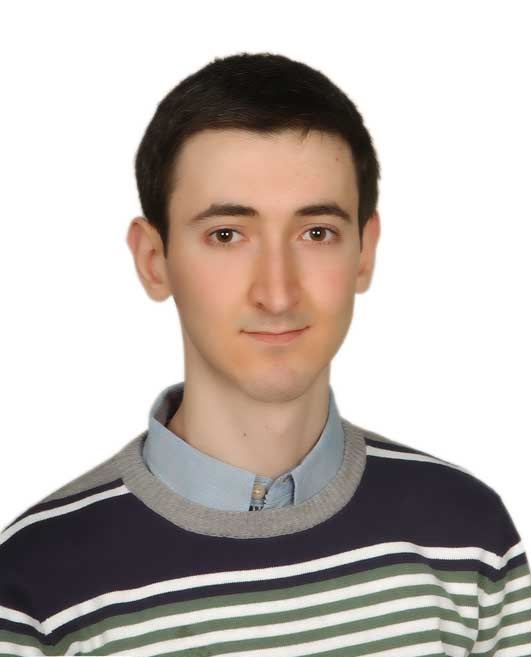
\includegraphics[scale=0.75,keepaspectratio=true]{./fig/cv_photo}
 % photo.eps: 0x0 pixel, 300dpi, 0.00x0.00 cm, bb=14 14 279 359
\end{figure}

\end{textblock}
\textbf{Name Surname:} Tu\u{g}rul Yata\u{g}an\\

\vspace{-3mm}
\textbf{Place and Date of Birth:} Denizli / Turkey, 1992\\

\vspace{-3mm}
\textbf{E-Mail:} yatagan@itu.edu.tr\\


\textbf{EDUCATION:} 
\vspace{-3mm}
\begin{itemize}
  \item \textbf{B.Sc.:} 2015, Istanbul Technical University, Computer and Informatics Faculty, Computer Engineering Department
  \item \textbf{High School:} 2010, Denizli Nalan Kaynak Anatolian High School
\end{itemize}

\textbf{PROFESSIONAL EXPERIENCE:}   
\vspace{-3mm}
\begin{itemize}
  \item 2017-Present Embedded Software Engineer at Maxim Integrated
  \item 2015-2016 Software Engineer at AirTies Wireless Networks
  \item 2014 Software Development Summer Intern at Yeni Hayat IT Corp.
  \item 2013 Software Development Summer Intern at Kartaca IT Corp.
\end{itemize}

\textbf{PUBLICATIONS:} 
\vspace{-3mm}
\begin{itemize}
   \item Yatagan, T. and Oktug S., 2019, Smart Spreading Factor Assignment for LoRaWANs, 
   \textit{2019 IEEE Symposium on Computers and Communications (IEEE ISCC 2019)}
\end{itemize}

\vspace{-3mm}
% ---------------------------------------------------------------- %
% Fotografli ve yayin listeli (yayini varsa) ozgecmis onerilir.    %
% Fotograf ve adres sart degildir.				   %
% ---------------------------------------------------------------- %